\subsection{All rules across attacks and conditions}\label{sec:compare}

Figure~\ref{fig:compare} gathers the compromise results for every signature-free rule in four settings:
strong shared drift with all attacker types, the classic boundary poisoner, poison hidden in the clean
core, and a one-model botnet with two of three cameras infected. Table~\ref{tab:compare} gives the
numbers and the false alarms that each rule pays.

\begin{figure*}[t]
\centering
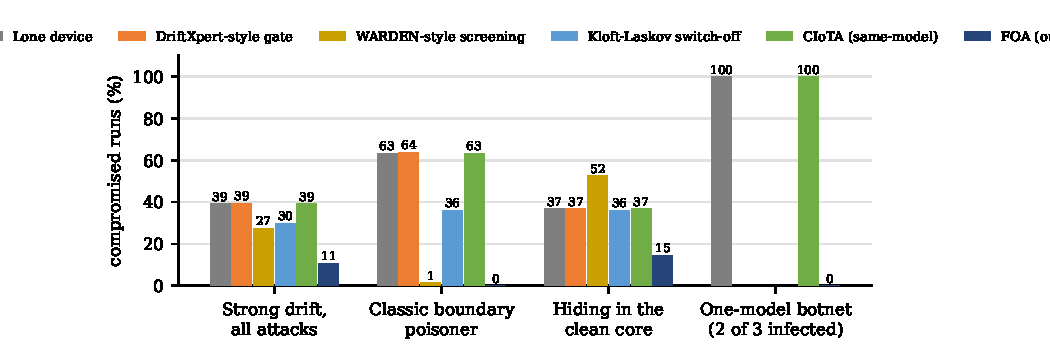
\includegraphics[width=\textwidth]{figures/fig_compare.pdf}
\caption{Compromised runs (\%) for each rule. Drift settings: 7 victims, 4 attacker shares, 10 held-out
seeds (840 runs per rule). Botnet: strong drift, 2 of 3 same-model cameras infected. Missing bars were not
run in that setting. CIoTA-style equals the lone device under drift because the nine-device fleet has
no three devices of one model, so it has no one to vote with.}\label{fig:compare}
\end{figure*}

\begin{figure*}[t]
\centering
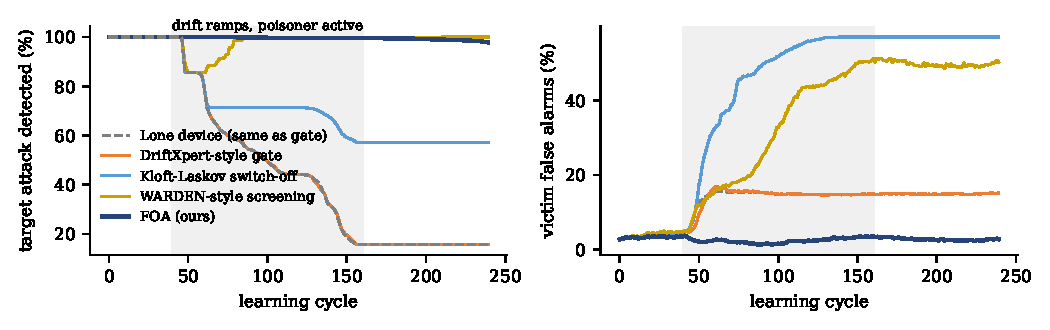
\includegraphics[width=\textwidth]{figures/fig_frog.pdf}
\caption{The boiling frog in action: classic boundary poisoner at share 0.3 during strong shared drift
(shaded: drift ramps and the poisoner is active), mean over 7 victims and 10 held-out seeds. Left:
share of the target attack still detected. Right: victim false alarms. The lone device (dashed) and the
outlier-ratio gate coincide.}\label{fig:frog}
\end{figure*}

\begin{table}[t]
\caption{Compromised runs (\%) by setting, and fleet false alarms after strong honest drift (\%, Table~\ref{tab:liveness}). Lower is better. -- : not run}\label{tab:compare}
\centering\footnotesize\setlength{\tabcolsep}{3.2pt}
\begin{tabular}{@{}lrrrrr@{}}
\toprule
Rule & All & Bound. & Core & Botnet & FPR \\
\midrule
Naive & 35 & 83 & 18 & -- & 2.6 \\
Single device & 39 & 63 & 37 & 100 & 24.6 \\
Outlier-ratio gate & 39 & 64 & 37 & -- & 24.6 \\
Alarm switch-off & 30 & 36 & 36 & -- & 45.0 \\
Clipping & 30 & 14 & 46 & -- & 55.9 \\
Frozen reserve & 27 & 1 & 52 & -- & 59.3 \\
CIoTA-style & 39 & 63 & 37 & 100 & -- \\
\textbf{FOA} & \textbf{11} & \textbf{0} & \textbf{15} & \textbf{0} & \textbf{9.0} \\
\midrule
TOA (oracle) & 5 & 0 & 10 & -- & 38.3 \\
\bottomrule
\end{tabular}
\end{table}

\textbf{Reading the comparison.} Among rules that do not know the attack in advance, FOA has the lowest
compromise rate overall (11\% against 27\% to 39\%), is never compromised by the boundary poisoner or by
the one-model botnet, and has the lowest rate for poison hidden in the clean core (15\%). The defences
that come closest on one attack pay elsewhere: the frozen reserve stops the boundary poisoner (1\%) but
is compromised in 52\% of core runs and raises 59\% false alarms; the alarm switch-off and clipping trade
safety for 45\% to 56\% false alarms. Only TOA is safer, and only because it is given the attack's
signature. Under the mimicry attacker, who imitates the shared drift, FOA (18\%) is not better than a lone
device (18\%) and the naive rule (2\%) does best (Table~\ref{tab:e3}); this is the case
Proposition~\ref{prop:frontier} predicts, because that attacker hides inside change the neighbours do see.

\begin{table}[t]
\caption{Outcome of each hypothesis}\label{tab:hyp}
\centering\footnotesize
\begin{tabular}{@{}p{1.25cm}p{4.7cm}p{1.45cm}@{}}
\toprule
Hypothesis & Evidence & Outcome \\
\midrule
H1 safety & 10.8\% compromised vs 39.2\% (single device) and 27\% to 30\% (gated); 9.4\% vs 43.1\% with the floor & Supported \\
H2 tracking & With the floor, 2.5\% fleet false alarms after strong drift vs 0.8\% for a single device & Supported \\
H3 cost & 1.2 to 1.9\,ms to combine, 92-byte frames, extra energy below sensor resolution on ESP8266 & Supported \\
H4 robustness & One-model botnet 0\% vs 100\% (same-model voting); decoys leave FOA's trajectory unchanged & Supported \\
\bottomrule
\end{tabular}
\end{table}
